%%%%%%%%%%%%%%%%%%%%%%%%%%%%%%%%%%%%%%%%%%%%%%%%%%%%%%%%%%%%%%%%%%%%%%%%%%%%%%%%
%2345678901234567890123456789012345678901234567890123456789012345678901234567890
%        1         2         3         4         5         6         7         8

\documentclass[letterpaper, 10pt, conference]{ieeeconf} 

%\documentclass[a4paper, 10pt, conference]{ieeeconf}      % Use this line for a4 paper

\IEEEoverridecommandlockouts                              % This command is only needed if 
                                                          % you want to use the \thanks command

\overrideIEEEmargins                                      % Needed to meet printer requirements.

\usepackage[utf8x]{inputenc}
\usepackage{graphicx}

%\usepackage{tikz}
%\usetikzlibrary{graphs,graphdrawing,arrows}
%\usegdlibrary{trees, layered}
\usepackage[bookmarks=true]{hyperref}

\usepackage{xspace}
\newcommand{\eg}{e.g.,\xspace}
\newcommand{\etal}{et al.\xspace}
\newcommand{\ie}{i.e.,\xspace}
\newcommand{\etc}{etc.\xspace}
\newcommand{\vs}{vs.\xspace}
\newcommand{\resp}{\textit{resp.}\xspace}
\newcommand{\cf}{cf.\xspace}

\newcommand{\uwds}{{\sc underworlds}\xspace}


\usepackage{amssymb}
\usepackage{amsmath}
\DeclareMathOperator{\op}{\odot}
\DeclareMathOperator{\filter}{\otimes}
\DeclareMathOperator{\generator}{\oplus}
\DeclareMathOperator{\consumer}{\ominus}
\DeclareMathOperator{\W}{\mathcal{W}}
\DeclareMathOperator{\Ws}{\boldsymbol{W}}
\DeclareMathOperator{\Os}{\boldsymbol{O}}


\graphicspath{{figs/}}

\usepackage[cache]{minted}
\renewcommand{\theFancyVerbLine}{
  \sffamily\textcolor[rgb]{0.5,0.5,0.5}{\scriptsize\arabic{FancyVerbLine}}}

\newminted{python}{frame=lines,
                    linenos=true,
                    fontsize=\scriptsize,
                    xleftmargin=1.8em}

\newmintinline[python]{python}{fontsize=\footnotesize}


\begin{document}

\title{\LARGE \bf
{\sc underworlds}: Cascading Situation Assessment for Robots
}


\author{Séverin Lemaignan$^{1}$, Yoan Sallami$^{2}$, Christopher Wallbridge$^{1}$, Aurélie Clodic$^{2}$ and Rachid Alami$^{2}$%
\thanks{$^{1}$Authors are with Centre for Robotics and Neural Systems,
        Plymouth University, Plymouth PL48AA, United Kingdom
        {\tt\small firstname.surname@plymouth.ac.uk},
	$^{2}$Authors are with LAAS-CNRS, Université de Toulouse, CNRS, Toulouse, France
        {\tt\small firstname.surname@laas.fr}}%
}




%%%%%%%%%%%%%%%%%%%%%%%%%%%%%%%%%%%%%%%%%%%%%%%%%%%%%%%%%%%%%%%%%%%%%%%%%%%%%%%%
\maketitle
\thispagestyle{empty}
\pagestyle{empty}

\begin{abstract}

    We introduce \uwds, a novel lightweight framework for \emph{cascading
    spatio-temporal situation assessment} in robotics. \uwds allows programmers
    to represent the robot's environment as real-time distributed data
    structures, containing both scene graphs (for representation of 3D
    geometries) and timelines (for representation of temporal events). \uwds
    supports \emph{cascading} representations: the environment is viewed as a
    set of \emph{worlds} that can each have different spatial and temporal
    granularities, and may inherit from each other.  \uwds also provides a set of
    high-level client libraries and tools to introspect and manipulate the
    environment models.

    This article presents the design and architecture of this open-source tool,
    and explores some applications, along with examples of use.

\end{abstract}


%%%%%%%%%%%%%%%%%%%%%%%%%%%%%%%%%%%%%%%%%%%%%%%%%%%%%%%%%%%%%%%%%%%%%%%%%%%%%%%%
\section{Introduction}


\uwds is a distributed and lightweight open-source
framework\footnote{\url{https://github.com/underworlds-robot/underworlds}} that
enables robot programmers to build and refine spatial and temporal
models of the environment surrounding a robot in real-time. \uwds makes it possible to share
these world models amongst the software components running on the robot.
Additionally, \uwds enables users to represent and manipulate
\emph{multiple alternatives} to the current, perceived world model in a distributed manner. For
instance, the world with some objects filtered out; the world `viewed' from the
perspective of another agent; a hypothetical world resulting from the simulated
application of a plan, etc.


\subsection{Distributed Situation Assessment}

\begin{figure}[ht!]
    \centering
    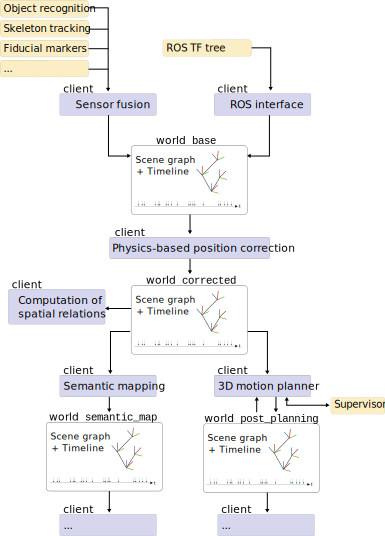
\includegraphics[width=\linewidth]{overview}
    \caption{Schema of a possible \uwds network: eight \emph{clients} (user-written \&
    architecture specific; in blue) are sharing environment
    models through four independent \emph{worlds} (made from joint spatial and
    temporal models). This architecture enables successive and modular
    refinement of the models (\emph{cascading} situation assessment),
    effectively adapted to each client's needs.}

    \label{fig|scene}

\end{figure}


Anchoring perceptions in a symbolic model suitable for decision-making requires
perception abilities and their symbolic interpretation. We call \emph{physical
situation assessment} the cognitive skill that a robot exhibits when it
represents and assesses the nature and content of its surroundings and monitors
its evolution.

Numerous approaches exist, like amodal (in the sense of modality-independent)
\emph{proxies}~\cite{Jacobsson2008}, grounded amodal
representations~\cite{Mavridis2006}, semantic
maps~\cite{Nuechter2008, Galindo2008,Blodow2011} or affordance-based planning
and object classification~\cite{Lorken2008, Varadarajan2011}.


\uwds is specifically inspired by geometric and temporal reasoners like {\sc Spark}
(\emph{SPAtial Reasoning \& Knowledge})~\cite{sisbot2011situation}.  {\sc Spark}
acts as a situation assessment reasoner that generates symbolic knowledge from
the geometry of the environment with respect to relations between objects,
robots and humans. It also takes into account the different perspective that
each agent has on the environment. {\sc Spark} embeds a modality-independent
geometric model of the environment that serves both as basis for the fusion of
the perception modalities and as bridge with the symbolic
layer~\cite{lemaignan2016artificial}. This geometric model is built from 3D CAD
models of the objects, furniture and robots, and full body, rigged models of
humans. It is updated at run-time by the robot's sensors.  Likewise, \uwds
embeds a grounded amodal model of the environment, updated online from the
robot's sensors (sensor fusion).

However, {\sc Spark} is a monolithic module that does not support sharing its
internal 3D model with other external components. In contrast, \uwds focuses on
offering a shared and distributed representation of the environment within the
robot's software architecture. This also distinguishes \uwds from complex
cognitive toolkits like KnowRob (as found in OpenEASE~\cite{beetz2015open}).
While these tools maintain a spatio-temporal model of the world, this model is
internal and not meant to be made widely accessible to other external processes.
\uwds focuses instead on re-usability and sharing of distributed spatio-temporal
models.  As such, \uwds can be seen as a middleware for spatio-temporal world
models and, contrary to KnowRob, it does \emph{not} provide any intrinsic high-level
processing or reasoning capability. Such reasoning skills are implemented in
loosely-coupled \emph{clients} (see Section~\ref{apiclients} hereafter).

Work on distributed scene graphs~\cite{naef2003blue} has been previously applied
to robotics to provide a shared 3D representation of the robot's environment
(for instance, the \emph{Robot Scene Graph}~\cite{blumenthal2013scene} or the
\emph{Deep State Representation} proposed in~\cite{bustos2016unified}).  \uwds
offers a similar distribution mechanism for 3D scene graphs and extends it to
temporal representations. Besides, \uwds further extends this line of work by
providing the ability to create, manipulate and share \emph{multiple alternative
worlds}. As an example, these could correspond to filtered or hypothetical
\emph{views} on the initial, perceived model of the environment.

\subsection{Representing Alternative States of the World}\label{alter}

The components which make use of spatial and temporal models of the environment
are usually found in the intermediate layers of robotic architectures, between
the low-level perceptual layers, and the high-level decisional layers. They
include modules like geometric reasoners (that compute spatial and topological
relations between objects), motion planners or action recognition modules.

These components exhibit different needs in terms of representation,
like different nominal spatial and/or temporal resolutions. For instance, a 3D
motion planner would typically use coarse 3D models of surrounding objects to
lower the computational load while planning, while a module assessing the
visibility of objects might need high-resolution models 
for accurate 3D visibility testing. This requirement of multiple
task-specific representations has been framed as the need for \emph{deep
representations} by Beetz~\cite{beetz2010towards}.

%Spatial models are also usually large as they might
%contain a lot of geometric data (including point clouds and meshes). Efficient
%real-time sharing of such datasets is non-trivial, particularly when the said
%data is changing (\eg in the case of map building or object recognition).

Traditional robotic middlewares, like ROS, are not particularly well suited to
deal with these different needs: full geometric data can be represented, but is
not first-class citizen: a basic task like displaying a 3D mesh at an arbitrary
position is not particularly easy to perform with ROS, requiring the combination
of static Collada meshes, a URDF kinematic description, TF broadcasters, and a
3D visualisation tool like RViz. Critically, simultaneously representing and
reasoning on alternative states of the environment is not directly feasible.

Representing alternative states is however often highly desirable. For instance,
software components manipulating environment models typically perform better if
the models are physically consistent. However, low-level perception inaccuracies
often introduce hard-to-avoid physical inconsistencies (like detected objects
floating in the air, or wrongly inset into other objects).
Therefore, a post-process stage (for instance, using a physics simulation
engine) is needed to move the objects seen by the robot into
physically-correct positions. Implemented with a classical approach (for
instance, using ROS TF frames), we would represent an object {\tt book} with two
frames: the original frame (\eg {\tt book\_frame\_raw}) and a second one
computed by the physics engine (\eg {\tt book\_frame\_corrected}). Such an
approach leads to the robot's 3D model being cluttered with multiple frames and
does not scale well.

Another example pertains to geometric task planning: a geometric task planner
typically needs to reason over hypothetical future states of the environment
(``What happens if I move this glass onto that pile of books?'').  The planner
generates many possible future states, which in turn might require further
processing (for instance, running a physics simulation). Such a tool would
benefit a flexible representation system, where models are derived from each
other, with partial modifications and different timescales.

A third example relates to human-robot interaction scenarios where \emph{perspective
taking} is important (a prototypical example being the game `I spy with my
little eye', as implemented in~\cite{ros2010which}). Perspective taking is a
cognitive skill that relies on the ability for an agent to take someone else's
point of view to estimate what they see from their perspectives. 
Perspective taking has previously been implemented in robotics by temporarily placing
virtual cameras at eye locations for each of the humans tracked by the
robot~\cite{ros2010solving}. While acceptable for simple cases, such an approach
does not maintain truly independent models of the environment for each
agent, and in particular does not permit false-belief
modelling~\cite{lemaignan2015mutual} whereas separate, independent world models
would effectively support such a skill.

Lastly, geometric \emph{pre-supposition accommodation} makes another interesting
case for alternative worlds representation. \emph{Pre-supposition accommodation}
originally comes from linguistics, where it describes the mechanism by which
\emph{context is adjusted [...] to accept [...] a sentence that imposes certain
requirements on the context in which it is
processed}~\cite{vonfintel2008presupposition}. In the context of spatio-temporal
representations, we call pre-supposition accommodation the ability of an agent
to adjust its model so that it matches some contextual constraint. For instance,
if A tells B to ``catch the red balloon behind you'', B might create a
representation of an imaginary red balloon, placed behind her, even without
actually observing the balloon: B \emph{accommodates} the \emph{pre-supposition}
of a red balloon being present behind herself. Endowing robots with this
capability has been touched upon by Mavridis~\etal within their multi-modal
\emph{Grounded Situation Model}~\cite{Mavridis2006}. However, to the best of our
knowledge, a general framework which would enable robots to accommodate spatial
and temporal pre-suppositions by deriving imaginary worlds from existing ones
has not been proposed so far.

\uwds addresses this need and the main contribution of this work is a generic
approach to \textbf{represent and share multiple parallel representations of the
world}. \uwds does so by allowing clients to clone existing worlds, modify
them, and re-share them, without the cost of duplicating geometric data (as
explained in section~\ref{design}). By organising clients in a network
(Figure~\ref{fig|scene}), worlds can be made dependent on each other, resulting
in a loosely-coupled modular approach to spatio-temporal world representation
that we call \emph{cascading situation assessment}.


\section{Design and Architecture}
\label{design}

%\subsection{Formal description}
%
%An \uwds \emph{world} $\W^k \in \Ws$ consists in a pair (\emph{scene}, \emph{timeline}),
%noted $\{\mathcal{S}^k,
%\mathcal{T}^k\}$.
%
%$\mathcal{S}^k=\{N^k, T^k\}$ is a tree representing a spatial scene (\emph{scene
%graph}), with $N^k$ the set of nodes and $T^k$ the set of 6D geometric
%transformations between the nodes ($|T^k| = |N^k| - 1$). $n^k_0 \in N^k$ is
%called the \emph{root node} of the scene $\mathcal{S}^k$.
%
%$\mathcal{T}^k=\{Evt^k, Sit^k\}$ is the world's \emph{timeline}, consisting in a
%set of events $Evt^k$ (duration-less states) and a set of situations $Sit^k$
%(states with a start time and an option end time).
%
%\uwds \emph{operators} (noted $\op\colon \Ws^{0\ldots m} \rightarrow
%\Ws^{0\ldots n}$) transform one world into another. Examples of operators
%include \emph{filters} (noted $\filter$), a common type of unary, antiextensive
%transformations such as $\filter\W^k \subseteq \W^k$, and \emph{generators}
%(noted $\generator$), a class of nullary operators that are used to create new
%worlds (for instance, from perception routines).
%
%Finally, an \uwds \emph{network} $\mathcal{N} = \{\Ws, \Os\}$ is a directed graph (cycles are
%permitted) of worlds $\Ws=\{\W^k\}, k\in0\ldots n$ and operators
%$\Os=\{\op^l\}, l \in 0\ldots m$. As described in the following sections,
%operators are typically implemented as independent software processes that connect at
%runtime to their operands, \ie the \uwds worlds, to read and write them. These
%processes are hereafter called \emph{clients} of the \uwds network.

%As an example, Figure~\ref{fig|formal-net} shows the
%formal model of the \uwds network represented in Figure~\ref{fig|scene}.
%
%\begin{figure}[!h]
%    \centering
%    \begin{tikzpicture}[nodes={text height=0.4cm,align=center,text width=1.5cm,
%                    draw=black!20, thick, fill=white, font=\footnotesize},
%                        tr/.style={draw=none,text width=0.3cm},
%                        >=stealth', rounded corners, semithick]
%\graph [layered layout, grow=right, level distance=0.5cm, sibling sep=.5em, sibling distance=1cm] {
%    "$\W^0$ {\tiny\tt base}" -- "$\filter^0$"[tr] -> "$\W^1$ {\tiny\tt corrected}";
%        "$\W^1$ {\tiny\tt corrected}" -- "$\op^2$"[tr] -> "$\W^3$ {\tiny\tt post\_planning}";
%        "$\W^1$ {\tiny\tt corrected}" -- "$\op^1$"[tr] -> "$\W^2$ {\tiny\tt semantic\_mapping}";
%};
%\end{tikzpicture}
%\caption{}
%    \label{fig|formal-net}
%\end{figure}
%


\subsection{Software architecture}

Figure~\ref{fig|scene} depicts a typical \uwds topology: a graph (that happens
to be an \emph{acyclic} graph on Figure~\ref{fig|scene}, but does not have to
be in the general case) of worlds, with clients connecting the worlds to each
others.
%In the following, we however tend to adopt a software engineering perspective,
%in which the \uwds network is made of \emph{clients} (which implement the
%operators) connected through shared data structures called \emph{worlds}.
%The formal model and this engineering-oriented model are isomorphic.

\subsubsection{Clients}

Software components implementing accessing \uwds worlds are
called clients. 
Clients can both read and write onto the worlds they are connected to, and
automatically see updates broadcast by other clients connected to the same
world. To ensure data consistency, worlds can have many simultaneous readers,
but only one writer at a given time.

\uwds provides several standard clients (like a 3D visualisation tool or a
physics engine simulator). Clients are however typically written by the end
users, depending on the needs of one's specific architecture.

%Three specific types of clients can be distinguished: \textbf{generator
%clients} which implement generator operators, and create and update worlds
%(`write-only' client, like the \emph{Sensor fusion} and \emph{ROS interface}
%clients in Figure~\ref{fig|scene}); \textbf{leaf clients} which on the contrary
%only read worlds, without modifying them (like the \emph{Computation of spatial
%relations} client on Figure~\ref{fig|scene}); and \textbf{transformers} which
%transform one representation into another (like the \emph{Semantic mapping}
%client on Figure~\ref{fig|scene}). \textbf{Filters} are a specfic class of
%transformer clients that copy an input world into an output world, performing some
%filtering operation in-between (like the client \textit{Physics-based position
%correction}).

\subsubsection{Worlds}

Worlds are effectively distributed data structures composed of a scene graph
representing the 3D geometry of the environment, and a timeline storing temporal
events.

While each world is technically independent from all the others, dependencies
(and therefore, coupling) arise between worlds from the clients' connections.
For instance, filters effectively create a dependency between worlds. On
Figure~\ref{fig|scene}, the \textit{Physics-based position correction} client
creates a dependency between the world {\tt base} (which represents here the
result of raw sensor fusion) and the world {\tt corrected} which would be a
physically-consistent copy of {\tt base}.  As a result, an \uwds network can
also be seen as a dependency graph between worlds (where cyclic dependencies
are permissible).

This architecture enables what we call \emph{cascading situation assessment}:
independent software components (the clients) build, refine and share
successive models of the environment by a combination of
filtering/transformations steps and model branching. A change performed by one
client (for instance, a face tracker updates the pose of the human head) may
thereby \emph{cascade} to each of the downstream, dependent worlds.

\subsubsection{Scenes}

Worlds contain both a geometric model and a temporal model. The geometric
model is represented as a scene graph. The scene graph has a unique root node,
to which a tree of other nodes is parented.

Nodes in an \uwds scene graph have three possible types: \textbf{objects} that
represent concrete physical objects (typically with one or several associated 3D
meshes); \textbf{entities} that represent abstract entities like reference
frames or groups of objects; \textbf{perspectives} that represent viewpoints
of the scene (like cameras or human gaze).
%; and \textbf{fields} that represent
%scalar or vector fields (like the visibility of an object, the working space of
%robot, \etc -- note that fields are not yet implemented in the current version
%of \uwds, see section~\ref{futurework}).

Every node has a unique ID, a parent, a 3D transformation relative to the parent
and an optional name. \emph{Object} nodes optionally store as well pointers to
their associated meshes. Importantly, mesh data (or other geometric datasets
like point clouds) are \emph{not} stored within the nodes themselves. \uwds
represents geometric data as immutable data, identified by their hash value
(preventing \textit{de facto} data duplication).  Nodes only store the hash
corresponding to the desired geometric data, and the actual data is pulled from
the server by the clients whenever they actually need it (for rendering for
instance).

\subsubsection{Timelines}

Complementing the spatial representation encapsulated in the scene graph, each
world also stores the world's \emph{timeline}. This data structure is shared and
synchronised amongst the clients in the same way as the scene graph.  Clients
can record and query both \emph{events} (duration-less states) and \emph{situations} in
the timeline, \ie states with a start time and a (possibly open-ended) end time.

%Importantly, the \uwds server automatically generates a snapshot of
%the scene graph whenever an event or situation is added to the timeline. The
%snapshot is associated to the event, which allows clients to effectively retrieve past
%states of the world. This capability is anticipated to be primarily used by \uwds clients
%performing action recognition.

\begin{figure}
    \centering
    \includegraphics[width=\linewidth]{uwds-screenshot}
    \caption{Screenshot of the {\tt uwds view} 3D visualisation and manipulation
    client. In this particular example, the 3D meshes have been pre-loaded using
    {\tt uwds load}. Their positions are then updated at run-time using the
    robot's sensors and proprioception (joint state).}
    \label{fig|uwds-view}
\end{figure}

\subsection{Distributed spatio-temporal models}
\label{arch}

\uwds is not a monolithic piece of software. Instead, it stands for both a
\emph{network of interconnected clients} which manipulate spatial and temporal
models of the robot environment (for instance, a motion planner, a object
detection module, a human skeleton tracker, etc.), and for a {client library}
that makes it possible to interface existing software components with the network.

Critically, the network is essentially hidden to the client: from the user
perspective, the environment model is manipulated as a local data structure (see
Listing~\ref{lst|pythonapi}). Modifications to the model are asynchronously synchronised with
a central server (the {\tt underworlded} daemon) and broadcast to every other
client connected to the same world.

As previously mentioned, worlds are composite data structures comprised of a
scene graph and a timeline. These data structures are synchronised using
Google's gRPC message passing framework\footnote{\url{http://www.grpc.io/}}, ensuring
high throughput, reliability and cross-platform/cross-language support. The \uwds
API is specifically discussed hereafter, in section~\ref{api}.


\uwds is meant to broadcast complex environment representations (typically
including large geometric datasets, like meshes) in real-time. \uwds itself does
not perform many CPU intensive tasks (CPU intensive processing tasks -- sensor
fusion, physics simulation, \etc -- are performed by the clients themselves) and
as such, the performance bottleneck is essentially the network's data
throughput.  In that regard, one of the simple yet critical optimisations
performed by \uwds is automatic caching of mesh data. Mesh data are not
transmitted when nodes are updated; only a hash value of the mesh data. The
client can then request the full data whenever it is actually needed.


\subsection{Time and space complexity analysis}

\uwds is fundamentally about distributing two datastructures: a scene graph
(with nodes representing spatial entities) and a timeline (where events are
stored as a flat list). Typical time and space complexities arise from these
datastructures. In typical usage scenarios (where the number of nodes or events
remain relatively small), the computational load to manipulate these
datastructures is however dominated by the actual processings performed by the
clients with the data.

More interesting is the time complexity of distributing changes across an \uwds
network. With $n$ the number of worlds and $m$ the number of clients in an \uwds
network, the worst-case (when every world is a parameter of every
client) time complexity of creating or updating a node and propagating the
change across the network is $O(n \times m)$ (this effectively corresponds to
the \uwds server performing $n \times m$ requests to notify clients of the
update).  The space complexity is the same (as clients own a full copy of the
worlds they monitor), except for mesh data whose space and time complexities are
$O(1)$ (only the server stores the mesh data).

In the common case of one client performing a full update of a single world
(with $p$ nodes) at each time step, the complexity of propagating these changes across
the network would be $O(p \times m)$. Figure~\ref{fig|performances} shows
measured propagation time for one change across up to 20 cascading worlds.

\begin{figure}
    \centering
    \includegraphics[width=\linewidth]{performances}
    \caption{Propagation times of one change (node creation)
    across $n$ worlds. The test is performed by running $n-1$ pass-through
    filters that monitor one world and replicate
    any changes into the next world. Durations measured over 20 runs, performed on
    a 8 core machine.}
    \label{fig|performances}
\end{figure}

\section{API \& Clients}
\label{apiclients}

\subsection{API}
\label{api}

As mentioned, \uwds uses Google's gRPC as message passing protocol. The protocol
is explicitly defined (using the \emph{protocol
buffers}\footnote{\url{https://developers.google.com/protocol-buffers/}}
interface definition language), and bindings to various languages and platforms
can be automatically generated from the protocol definition file (as of Jan
2018, gRPC can generate bindings for C, C++, C\#, Node.js, PHP, Ruby, Python, Go
and Java, on Windows, Mac, Linux and Android).  The cross-platform/cross-language support
of gRPC is especially welcome in the academic context, as it offers ease and
flexibility to plug a variety of pre-existing components into an \uwds network.


However, the gRPC message passing layer is low-level with respect to the typical
use of \uwds (manipulation of asynchronous, distributed spatio-temporal models
of the robot environment). In particular, the asynchronous fetching (and
conversely, remote updating) of nodes and time-related objects is typically
hidden from the user, and managed instead by the \uwds client library.

\uwds currently offers such a high-level client library for Python only (a C++
library is under development).  Listing~\ref{lst|pythonapi} gives a complete
example of an \uwds client performing simple filtering: the client continuously
listens for changes in an input world, removes some objects (in this case, items
whose volume is below a threshold), and forwards all other changes to
an output world, effectively making the output world a copy of the input world
with all smaller objects removed.

\begin{listing}[h!]

\begin{pythoncode}
import underworlds

# by default, connect to the server on localhost
with underworlds.Context("small_object_filter") as ctx:

    in_world = ctx.worlds["world1"]
    out_world = ctx.worlds["world2"]

    while True:

        in_world.scene.waitforchanges()

        for node in in_world.scene.nodes:
            if node.volume > THRESHOLD:
                out_world.scene.nodes.update(node)


\end{pythoncode}
    \caption{Example of a simple yet complete \uwds filter, written in Python:
    the client connects to the \uwds network, blocks until the world {\tt
    example\_in} changes, and only propagate nodes that match the condition to
    the world {\tt example\_out}.}

    \label{lst|pythonapi}
\end{listing}

\subsection{Standard Clients}
\label{std_clients}

The \uwds package provides several standard clients to perform common tasks on
\uwds networks.

\subsubsection{3D Visualisation and manipulation}

Interestingly, while \uwds deals with 3D geometries and scenes, it does
represent 3D entities purely as data structures; no visual representation is
involved (and as such, the \uwds server and core libraries do not depend on any
graphics library like OpenGL). However, for all practical purposes, the ability
to visualise the content of a scene is desirable. \uwds provides a standard
client, {\tt uwds view}, that performs real-time 3D rendering of worlds,
using OpenGL (Figure~\ref{fig|uwds-view}).

This tool also supports basic object manipulations (translations, rotations),
that are broadcast to the other \uwds clients connected to the same world.

\paragraph*{Assets loading}

%Geometric data like meshes can be loaded into a world (or rather, into the whole
%network as geometric data are treated as immutable resources shared amongst all
%worlds) by simply sending an array of vertices and faces to the \uwds server.
%As such, any client can load 3D data that is automatically made available to the
%whole network. For example, an object recognition module recognises a new
%object. It sends the mesh to the \uwds server and creates a new node which
%references the mesh. At the next frame update, the 3D viewer sees a new node
%referencing an unknown mesh. The viewer requests the mesh data from the
%server, stores it internally (\eg as an OpenGL buffer), and renders it. Whenever
%the node transformation is updated, the 3D viewer can re-render the node without
%having to download the mesh from the server again.

Often, objects manipulated by the robot have known meshes with corresponding CAD
models that can be conveniently pre-loaded. In these cases, \uwds provides a
tool, {\tt uwds load}, that loads a mesh into a \uwds network (and optionally,
creates a node) from a large range of 3D formats (including Collada, FBX, OBJ,
Blender)\footnote{The underlying import
capability is provided by the {\sc assimp} library.
\url{http://assimp.sourceforge.net/}}.

\subsubsection{Physics simulation}\label{physics}

When perception modules provide objects localization, the consistency is not guarantee, objects on a table seem to slightly flight in the air, when dropping them in a bin the localization is not updated any more when the objects are occulted, resulting in objects that fly just above the bin.

Being able to manage that issues by simulating the gravity is the purpose of a dedicated client  
{\tt physics filter} that have been designed using Bullet RT physics simulation and pybullet \url{https://pybullet.org/} library, it provides from an input world, an output world where objects described by an URDF file are filtered by the simulator, which gives us the near future of the objects based on their position, mass and inertia.

\subsubsection{Introspection and debugging}

\uwds provides a range of tools to inspect a running network. Graphical
tools ({\tt uwds explorer} and {\tt uwds timeline}, see Figure~\ref{fig|explorer})
provide a user-friendly overview of the system's graph with the connections
between the clients and the worlds, as well as their activity.

\begin{figure}
    \centering
    \includegraphics[width=\linewidth]{tools}
    \caption{Screenshots of the timeline (top) and network (bottom)
    introspection tools. Worlds are represented as boxes; clients as ellipses.}
    \label{fig|explorer}
\end{figure}

Specialised command-line tools are also available to list the worlds
and their content ({\tt uwds ls}) at run-time, or to display detailed information for a
specific node ({\tt uwds show}).

\subsubsection{Interface with ROS}

\uwds is meant to integrate as easily as possible into existing robot
architectures, and interfaces transparently with ROS' TF frame system through
the {\tt uwds tf} client.

The {\tt uwds tf} client continuously monitors the ROS TF tree, and mirrors
TF frames as nodes in the desired \uwds world. A node is first created if none
matches a given TF frame, and its transformation is subsequently updated,
mirroring the TF frame. A regular expression can be provided to only mirror a
subset of the TF tree into \uwds.

Currently, the process is unidirectional: the {\tt uwds tf} client performs TF
to \uwds updates, but not the reverse.

\subsection{Spatial Reasoning and Perspective Taking}

Spatial reasoning~\cite{O'Keefe1999} is a field in its own right, and has been
used for natural language processing for applications such as direction
recognition~\cite{Kollar2010,Matuszek2010} or language
grounding~\cite{Tellex2010}. Other examples in human-robot interaction include Ros
\etal~\cite{ros2010solving, ros2010which} which has recently been integrated
into a full architecture for autonomous human-robot
interaction~\cite{lemaignan2016artificial}.

\begin{figure}
    \centering
    \includegraphics[width=\linewidth]{spatialrelations}
    \caption{The {\tt spatial\_relations} client computes perspective-aware
    spatial relations between objects and agents: \emph{allo-centric} relations (like
    {\tt is in} or {\tt is on}) are independent of the viewpoint, while
    \emph{ego-centric} relations ({\tt in front of}, {\tt left of}) depend on
    the viewer perspective.}
    \label{fig|spatialrelations}
\end{figure}

\uwds provides an exemplary client ({\tt spatial\_relations}) to compute both
allo-centric and ego-centric (\ie viewer-dependent) spatial relations
between objects (Figure~\ref{fig|spatialrelations}).
Other libraries, like QSRLib~\cite{gatsoulis2016qsrlib}, that implement
computational models of Qualitative Spatial Relations could be trivially
combined with \uwds to provide more advanced geometric analysis.


\uwds also implements an efficient algorithm to assess object visibility from a
specific viewpoint (\ie from a given \emph{perspective} node). The algorithm (color
picking) enables fast (single pass) computation of the visibility of every
object in the scene, while providing control regarding how many pixels should be actually
visible for the object to be considered globally visible. The
command-line tool {\tt uwds visibility} returns the list of visible objects from
the point of view of each camera in a given world, and \uwds also provides the
helper class {\tt VisibilityMonitor} to programmatically access visibility
information.

When integrated into a filter node, visibility computation allows easy
creation of new worlds representing the estimated perspectives of the different
agents.
%Listing~\ref{lst|humanperspective} provides the complete code of such an
%\uwds client.

%
%\begin{listing}[h!]
%\begin{pythoncode}
%import copy
%import underworlds
%from underworlds.tools.visibility import VisibilityMonitor
%
%with underworlds.Context("Human PoV") as ctx:
%
%    source = ctx.worlds["base"]
%    target = ctx.worlds["human_perspective"]
%
%    # pick up the first node named 'human'
%    human = source.scene.nodebyname("human")[0]
%    target.scene.nodes.append(human)
%
%    # VisibilityMonitor computes the set of visible 
%    # nodes from a given viewpoint
%    visibility = VisibilityMonitor(ctx, source)
%
%    node_mapping = {}
%
%    while True:
%
%        for node in visibility.from_camera(human):
%
%            newnode = node.copy()
%
%            # track the correspondence between nodes
%            # in source and target scenes
%            if node in node_mapping:
%                newnode.id = node_mapping[node].id
%            else:
%                node_mapping[node] = newnode
%
%            # reparent the nodes to the new root
%            if node.parent == source.scene.rootnode.id:
%                newnode.parent = target.scene.rootnode.id
%
%            target.scene.nodes.update(newnode)
%
%        source.scene.waitforchanges()
%
%\end{pythoncode}
%    \caption{Example of an \uwds client that creates a world named {\tt
%    human\_perspective} from a source world {\tt base} by only updating objects
%    that are in the field of view of the human. As such, {\tt human\_perspective} is
%    a real-time model of the human perspective on the scene.}
%
%    \label{lst|humanperspective}
%\end{listing}
%

\section{Application Example}
\label{application}

\subsection{Application to human-robot interaction and spatial reasoning}

\begin{figure}
    \centering
    \includegraphics[width=\linewidth]{l2tor-photo2-blind}
    \caption{A user manipulating objects on top of an RFID mat (providing object
    localisation) with a NAO robot, while an operator monitors
    the interaction on a tablet that displays an {\tt uwds view} client [photo blurred for blind review].}

    \label{fig|l2torexample}
\end{figure}

\uwds has been used within the European L2TOR project~\cite{belpaeme2015l2tor}
in order to conceptualise and visualise the spatial relations and visibility of
the physical objects that participants interact with. In one of the scenarios of this
project, participants are instructed by a NAO robot to manipulate a number of
Duplo-like animals on top of a printed background paper which serves as a
landscape (Figure~\ref{fig|l2torexample}). The robot instructions are based on
pedagogical strategies to promote spatial relation learning by object
manipulation. Such instructions include commands to place the elephant
\textit{on top} or \textit{next to} the cube, or put the giraffe \textit{inside}
the house.  To assess the performance, the robot and the operator need to
compute spatial relationships between objects from the visual perspective of the
participant.



\subsection{Application to joint-action situations}

\uwds is used 
%within the European MuMMER project
to be able to assess visibility and knowledge about objects, places and agents within the scene.

Let's imagine a little example with two humans and a robot looking at a table. On the table there is an object that is only seen by one human and the robot (it is hidden for the second human). Figure~\ref{fig|mummerarchitecture} illustrates the topology of the \uwds network we can define for this example. 

\begin{figure}
    \centering
    \includegraphics[width=\linewidth]{l2tor-photo2-blind}
    \caption{TODO LAAS: update photo -> MuMMER picture?}
    \label{fig|mummer-example}
\end{figure}

%\uwds has been used within the European MuMMER project
%in order to conceptualise and visualise the spatial relations and visibility of
%the physical objects that participants interact with.


\begin{figure}
    \centering
    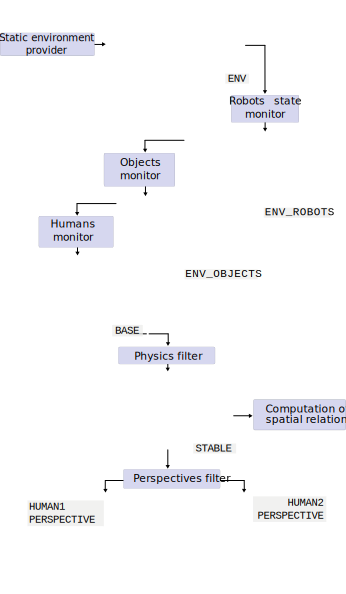
\includegraphics[width=\linewidth]{laasudws}
    \caption{TODO LAAS update archi -- Schema of the \uwds architecture used in
    the MuMMER project. }
    \label{fig|mummerarchitecture}
\end{figure}
%The interaction scenario requires a number of \uwds clients. The clients are
%distributed across...

A first client \textit{env\_provider} provides the environment set-up and allows to build a first \texttt{ENV} world where static objects/furnitures and walls are present. 
Then, the system cascades three worlds successively by the help of three clients. \textit{robot\_monitor} provides a first world where the robot is present. \textit{humans\_monitor} provides a new world where the humans are present (using~\cite{Khalidov_Idiap-RR-02-2017}). \textit{object\_monitor} provides a new world where the objects are present (using {\tt ar\_track\_alvar}\footnote{\url{http://wiki.ros.org/ar_track_alvar}}). At this end we obtain a world \texttt{BASE}.

This world \texttt{BASE} is then passed through a \textit{physics filter} client as explained in section~\ref{physics} to obtain a \texttt{STABLE} world where all elements are present and consistent: robot, humans, objects and static environment. On this world, we use \textit{Computation of spatial relations} client to get information such as {\tt onTop}, {\tt isIn} or {\tt isAbove}.

This world \texttt{STABLE} is then used by a \textit{perspective filter} client to provide different perspectives given the monitored agent (in our case: human 1, human 2 or the robot itself). Besides giving a view of the input world in the perspective of the monitored agent (through the robot's own perspective), it aggregates all the information visibly gathered by this agent. Consequently, it does not offer a snapshot of the agent belief at a particular time but an aggregated estimation along the time.

With this network, we are able to assess among other things that the object on the table is seen by the robot and human 1 but not by human 2. Moreover, if human 1 moves in a position where the object becomes not visible for him, the \textit{perspective filter} will keep the knowledge about the fact that he has already seen it (and keep the last position where it has been seen).

It has to be noticed that this knowledge could be wrong relatively to the current "real" state of the world, but it represents the monitored agent belief about the world.

%This knowledge could then be used by planner such as HATP to plan differently given the knowledge or ignorance of an agent regarding the environment.

We are currently setting up this kind of network in the framework of the European project MuMMER where a Pepper robot is intended to handle interactive situations in a Mall in Finland. One of the situation is a guiding task where Pepper will help people to find their route by pointing them landmarks and explaining them how to reach a destination. The use of \uwds enables to get knowledge about what the customer sees (or has seen) or not and to handle the task accordingly. We plan also to be able to add information coming from the dialogue (e.g. if the customer says that he has seen a particular landmark that could consequently be added to his belief world). Moreover, we plan also to use alternative world ability given by \uwds (as explained in \ref{alter}) (e.g. to create a world where we put the customer in front of the desired shop to infer (and be able to explain him) what he will see at destination).

\section{Discussion and Conclusion}

\subsection{Relation to existing robotic middleware}

Like traditional robotic middleware, \uwds offers a form of distributed
computation based on message passing. However, it distinguishes itself from
existing middleware in significant ways. Most importantly, \uwds purposefully
does not offer any \emph{general} capability to distribute computation and data
flow amongst independent components: it focusses specifically on distributing
environment models, both spatial (geometric models) and temporal (events and
situations). In that sense, \uwds really is a \emph{distributed datastructure}
that addresses the specific needs of spatio-temporal modelling,
including the modelling of hypothetical, alternative world models, something
that traditional middlewares like ROS do not address adequately.

While using standard middleware as \emph{underlying transport} for \uwds would be
technically feasible and relatively easy to implement, it does not offer any
clear advantage over lighter and dedicated message passing libraries like ZeroMQ
or gRPC (the later being the one used by \uwds).

\subsection{Future work}
\label{futurework}

As illustrated in section~\ref{application}, \uwds is already deployed and used
on the field. Several features are however still under development.

\subsubsection{Representation capabilities} as presented in
section~\ref{design}, the current version of \uwds allows to represent
\emph{objects}, \emph{abstract entities} like groups and \emph{perspectives}.
\emph{Fields} are also part of the \uwds design, but are not yet implemented.
Fields are commonly used to represent
continuously-valued spatial entities. Fields might or might not be spatially
bounded. Examples include the working space of a robot arm (spatially bounded),
the field of view of a camera (spatially bounded), proxemics (potentially
unbounded). We plan to represent fields in \uwds using the memory-efficient
octomaps~\cite{hornung2013octomap} or NDT-OM maps~\cite{saarinen20133d}.
Similarly to geometric data,these datastructures
will not be directly stored with the nodes (nodes will refer to them through 
handles), but unlike geometric data, they will not be treated as immutable
datasets by the server, permitting real-time updates.

\paragraph*{Representation of uncertainty} currently node positions are 
stored as $4\times4$ transformation matrices, relative to the node parent. This
representation is efficient, and conveniently matches traditional representation
systems (including ROS TF frames or OpenGL transformations). However, the explicit management
of uncertainties is instrumental to many robotic applications, and we plan to
add full support for position uncertainties to \uwds. We plan to add this
support by adding a pose covariance matrix to the nodes, and equipping the
different \uwds helper tools with corresponding support (like covariance
ellipses visualisation in {\tt uwds view}).


%\subsubsection{Manipulation of representations} \uwds makes it possible to
%cheaply clone and modify multiple worlds. However, little is provided to
%jointly manipulate sets of worlds. In that regard, we plan to add a mechanism to
%efficiently \emph{compare} two worlds. This would permit a client
%to quickly identify modifications applied to a world, and could prove especially
%useful when combined with temporal events to answer questions like ``what has
%changed in the scene?''. Comparisons between worlds involves the definition of
%an efficient fuzzy \emph{diff} algorithm for 3D scene graphs, able to
%selectively ignore non-relevant micro displacements.

\subsubsection{Implementation and Integration} we plan to continue to
improve the integration of \uwds into existing software architectures. A
short-term goal is to provide excellent C++ support, with a high-level,
user-friendly C++ client library. This is critical for a broader adoption of \uwds
within the robot community. Support for other languages might follow, depending
on demands and open-source contributions.

%In term of implementation, we are also investigating alternative back-ends that
%could compete with gRPC to provide the synchronisation mechanisms between
%clients. Due to the high-level nature of \uwds (a set of shared, tree-like data
%structures), the use of the GIT version control system is one particular (if
%unusual) option being studied. The scene graph would be represented as a
%hierarchy of directories, nodes would be files in these directories, creating
%new worlds would consist in creating a branch in the repository, and sharing
%would be supported through the usual pull/push GIT mechanisms. Initial
%prototyping shows that under the right conditions (in particular, an in-memory
%file system), performance is not an issue. Automatic conflicts resolution, on
%the other hand, might prove more challenging.


\subsection{Conclusion}

We have introduced \uwds, a novel framework for shared and composable
spatio-temporal representations of a robot's world. The key contributions of our
approach are: a composite data structure for environment representation within a
robotic software architecture, made of a scene graph and a timeline; a mechanism
to efficiently and transparently share this data structure amongst a set of
clients (the software modules of the robot); a cascading architecture permitting
the explicit of representation of alternative states of the world while
maintaining a network of dependencies.
%; a typology of clients
%(\emph{root}, \emph{leaf}, \emph{filter}, \emph{transformer}) to systematically
%describe such a network of representations dependencies.

We have additionally presented a concrete instantiation of a system relying on \uwds
for its representation needs, and we have sketched future directions of
development.

We believe this work can practically support existing robotic architectures with
state-of-the-art spatio-temporal representation capabilities. We also hope that
this line of research can lead to a better understanding of the representation
needs of modern robotic systems, and participate to the emergence of a possible
common representation platform for robots, building on previous formalisation
efforts like the RSG-DSL domain specific language~\cite{blumenthal2014towards}.

\section*{Acknowledgment}

This work has been supported by the EU H2020 Marie Sk\l odowska-Curie Actions
project DoRoThy (grant 657227),  the EU H2020 MuMMER project (grant 688147)
and the EU H2020 L2TOR project (grant 688014).


\bibliographystyle{IEEEtran}
\bibliography{bibliography}




\end{document}
